-\chapter{Time Evolutions}
In this chapter we will be looking a the conservative form of an equation. An equation is said to be in it's conservative form if it can be written as:
\begin{equation*}
  u_t + F(x,u)_x = 0
\end{equation*}
The advection and diffusion equations can therefore be written in conservative form, as well as Burger's equation.
%%%%%%%%%%%%%%%%%%%%%%%%%%%%%%%%%%%%%%%%%%%%%%%%%%%%%%%%%%%%%%
\section{Lax-Fredrichs}
The Lax-Fredrichs (LF) time evolutions scheme for conservative equation is given by:
\begin{equation*}
  v^{n+1}_j \simeq \frac{1}{2}(v^n_{j+1} + v^n_{j-1}) - \frac{k}{2h}(F^n_{j+1}-F^n_{j-1}) + O(k,h^2)
\end{equation*}
Focusing on the first term of the LF method, we see 
\begin{equation*}
  \frac{1}{2}(v^n_{j+1} + v^n_{j-1}) = v^n_j + \frac{1}{2}(v^n_{j+1} - 2v^n_j + v^n_{j-1})
\end{equation*}
If $F^n_j$ is then set to $cv^n_j$, we then get the centered Euler form of the advection equation with this second derivative component. This component then warps the advection equation to 
\begin{equation*}
 u_t + cu_x = \frac{h^2}{2k}u_{xx}
\end{equation*}
This gives the centered Euler a dissipative term, $\epsilon = \frac{h^2}{2k}$. Setting $\frac{h}{k}$ to be a constant, $\zeta$, we get
\begin{equation*}
  \epsilon = \frac{1}{2}\zeta h
\end{equation*}
Therefore as $h\rightarrow 0$, $\epsilon\rightarrow0$, and the exact form of the advection equation is formed. This is known as artificial dissipation and is used to stabilize an unstable scheme. It is also known as Kreiss-Oliger dissipation.
%%%%%%%%%%%%%%%%%%%%%%%%%%%%%%%%%%%%%%%%%%%%%%%%%%%%%%%%%%%%%
\section{Lax-Wendroff}
The Lax-Wendroff (LW) scheme uses the LF scheme to first obtain a ``half step'', which it then uses to perform a leapfrog=like step to achieve the next time step. The half steps are given as:
\begin{equation*}
  \begin{align}
  v^{n+1/2}_{j-1/2} &\simeq \frac{1}{2}(v^n_j + v^n_{j-1}) - \frac{k}{2h}(F^n_j-F^n_{j-1})\\
  v^{n+1/2}_{j+1/2} &\simeq \frac{1}{2}(v^n_{j+1} + v^n_j) - \frac{k}{2h}(F^n_{j+1}-F^n_j)\\
  \end{align}
\end{equation*}
And the leapfrog step is given as:
\begin{equation*}
  v^{n+1}_j \simeq v^n_j-\frac{k}{h}(F^{n+1/2}_{j+1/2}-F^{n+1/2}_{j-1/2})
\end{equation*}
The addition of this half step improves on the LF scheme from $O(h^2,k)$ to $O(h^2,k^2)$.
\\
\\
For the advection equation specifically, we can derive the LW scheme with $F$ set to $cu$ to obtain
\begin{equation*}
\begin{align}
  v^{n+1/2}_{j-1/2} &\simeq \frac{1}{2}(v^n_j + v^n_{j-1}) - \frac{ck}{2h}(v^n_j-v^n_{j-1})\\
  v^{n+1/2}_{j+1/2} &\simeq \frac{1}{2}(v^n_{j+1} + v^n_j) - \frac{ck}{2h}(v^n_{j+1}-v^n_j)\\
\end{align}
\end{equation*}
as the half steps. Therefore the full scheme is
\begin{equation*}
\begin{align}
  v^{n+1}_j &\simeq v^n_j-\frac{ck}{h}\big(\frac{1}{2}(v^n_j + v^n_{j-1}) - \frac{ck}{2h}(v^n_j-v^n_{j-1})- \frac{1}{2}(v^n_{j+1} + v^n_j) - \frac{ck}{2h}(v^n_{j+1}-v^n_j)\big)\\  
  v^{n+1}_j &\simeq v^n_j-\frac{ck}{2h}(v^n_{j+1} - v^n_{j-1}) + \frac{c^2k^2}{2h^2}(v^n_{j+1} -2v^n_j + v^n_{j-1})
\end{align}
\end{equation*}
We can see that this is similar to LF scheme for the advection equation, but with $\epsilon=c^2k^2/2$ as part of the dissipative term. Unlike the LF scheme however, the dissipative term is not dependent on $h$ which would result in a fixed $\zeta$, but rather, due to this, it may be subject to amplitude dissipation. We can check this by using Von Neumann analysis on the scheme.
\\
\\
Start by setting
\begin{equation*}
  v^n_j = \hat{v}^n(\omega)e^{i\omega hj}
\end{equation*}
substituting this into the LW scheme advection equation, we get
\begin{equation*}
\begin{align}
  \hat{v}^{n+1}e^{i\omega hj} &= \hat{v}^ne^{i\omega hj}-\frac{ck}{2h}(\hat{v}^ne^{i\omega h(j+1)} - \hat{v}^ne^{i\omega h(j-1)}) + \frac{c^2k^2}{2h^2}(\hat{v}^ne^{i\omega h(j+1)} -2\hat{v}^ne^{i\omega hj} + \hat{v}^ne^{i\omega h(j-1)}) \\
  \hat{Q}\hat{v}^ne^{i\omega hj} &= \hat{v}^ne^{i\omega hj} \big(1 - \frac{ck}{2h}(e^{i\omega h}+e^{-i\omega h}) + \frac{c^2k^2}{2h^2}(e^{i\omega h} -2+ e^{-i\omega h})\big)\\
  \hat{Q} &= 1 - \frac{ck}{2h}(e^{i\omega h}-e^{-i\omega h}) + \frac{c^2k^2}{2h^2}(e^{i\omega h} -2+ e^{-i\omega h})\\
  \hat{Q} &= 1 - i\frac{ck}{h}\sin\omega h - \frac{c^2k^2}{h^2}(1 - \cos\omega h)\\
\end{align}
\end{equation*}
Setting $\frac{ck}{h}=\alpha$ and solving for $||\hat{Q}||^2$, we get
\begin{equation*}
\begin{align}
  ||\hat{Q}||^2 &= (1 - \alpha^2(1 - \cos\omega h))^2 + (\alpha\sin\omega h)^2\\
  ||\hat{Q}||^2 &= 1 - 2\alpha^2(1 - \cos\omega h) + \alpha^4(1 - \cos\omega h)^2 + \alpha^2\sin^2\omega h\\
  ||\hat{Q}||^2 &= 1 + \alpha^2 \big( 2(1 - \cos\omega h) + \alpha^2(1 - \cos\omega h)^2 + \sin^2\omega h \big)\\
  ||\hat{Q}||^2 &= 1 + \alpha^2 ( 2 - 2\cos\omega h + \alpha^2(1 - \cos\omega h)^2 + 1 -\cos^2\omega h )\\
  ||\hat{Q}||^2 &= 1 + \alpha^2 \big( \alpha^2(1 - \cos\omega h)^2 - (\cos^2\omega h - 2\cos\omega h + 1) \big)\\
  ||\hat{Q}||^2 &= 1 - \alpha^2 (1 - \alpha^2)(1 - \cos\omega h)^2\\
\end{align}
\end{equation*}
Therefore
\begin{equation*}
\begin{align}
  ||\hat{Q}||^2 &\leq 1 \text{ so long as}\\
  1- \alpha^2 	&\leq 0 \\
  1	 	&\leq \alpha \\
  1		&\leq \frac{ck}{h} \\
  c		&\leq \frac{h}{k}
\end{align}
\end{equation*}
Which means that it is stable so long as Courant's stability condition is met.
\\
\\
Implementing this scheme with the advection equation of a Gaussian pulse with $c=1$ and $k=h$ and evolving the system over 4 units of time. Figure \ref{laxwen_adv} shows that the pulse is almost perfectly propagated by this method. The L2-norm of the error can be seen in Figure \ref{laxwen_adv_l2} showing that the method is very stable.
%------------------------------------------------------------------------------------------------------------------------------------------
\begin{figure}[H]
 \centering
 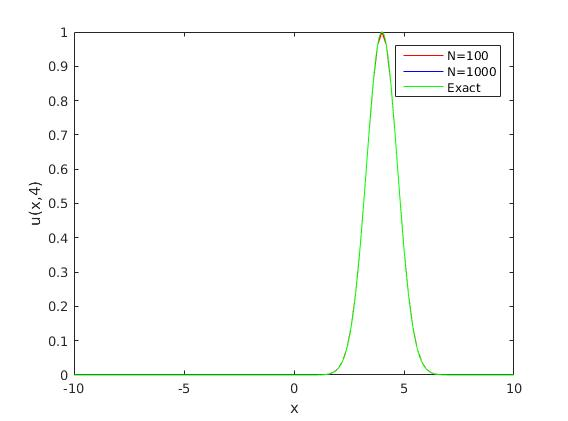
\includegraphics[scale=0.5]{Images/lw_adv_4.jpg}
 \caption{Lax-Wendroff Approximation after 4 seconds}
 \label{laxwen_adv}
\end{figure}
%------------------------------------------------------------------------------------------------------------------------------------------
\begin{figure}[H]
 \centering
 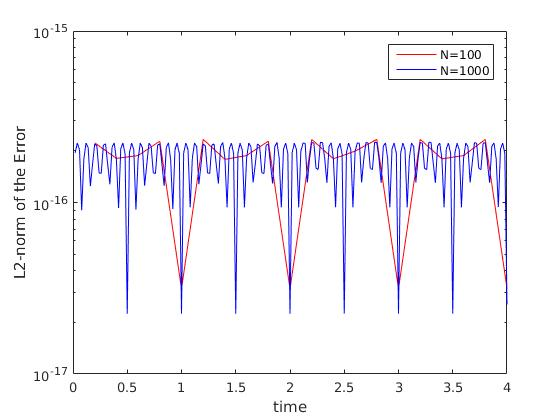
\includegraphics[scale=0.5]{Images/lw_adv_4_l2.jpg}
 \caption{L2 norm of the Error of Lax-Wendroff Approximation over 4 seconds}
 \label{laxwen_adv_l2}
\end{figure}
%------------------------------------------------------------------------------------------------------------------------------------------
Comparing the Lax-Wendroff to the centered leapfrog and upwind Euler, we find that it is more stable than both these methods



